\section{実験方法}
まず,平面のビッカース硬さ測定を行った.次に,直線運動型すべり摩擦試験機を用いて,大気中無潤滑下における球と平面の間の摩擦係数の測定を行い,接触形態と摩擦係数の関係を調査した.

\subsection{試験片}
ボール試験片として高炭素クロム軸受鋼(JIS SUJ2)球,プレート試験片としてアルミ合金(A5052)を用いた.それぞれの試験片の機械的性質を表\ref{tbl:試験片特性}に示す.また,ボール試験片,プレート試験片はそれぞれヘキサン中で5分間超音波洗浄し,デシケータ内で脱気したのち,実験に供した.

\begin{table}[htbp]
    \centering
    \caption{Mechanical properties of ball and plate specimens.} % 表のキャプション
    \label{tbl:試験片特性} % 参照用ラベル
    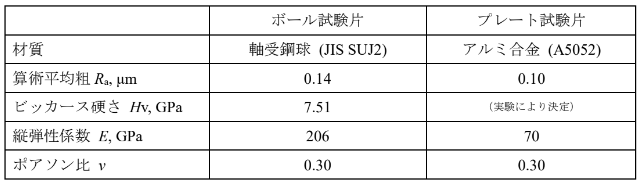
\includegraphics[width=0.8\textwidth]{fig/fig_試験片特性.png} % 画像ファイル名と幅を指定
\end{table}

\subsection{ビッカース硬さ試験方法}
プレート試験片のビッカース硬さの測定には,マイクロビッカース硬さ試験機を用いた.負荷重量を1kgf,荷重負荷時間を20sとし,圧痕の対角線長さからビッカース硬さを算出した.プレート試験片上において5点測定し,平均値及び標準偏差を求めた.

\subsection{摩擦試験方法}
図\ref{fig:fig_摩擦試験機}に摩擦係数測定のための試験装置の模式図を示す.ボール試験片\textcircled{\scriptsize 1}は,試験片ホルダーに装着したのち上部のアームに固定した.プレート試験片\textcircled{\scriptsize 2}は下部のステージ\textcircled{\scriptsize 4}に固定した.錘\textcircled{\scriptsize 3}により一定の荷重を加え,下部ステージを任意のすべり速度で直線運動させることにより,すべり摩擦を行った.このとき,摩擦力は上部のアームに取り付けられたロードセル\textcircled{\scriptsize 5}により検出され,PCに記録された.なお,ステージの移動には加速と減速が伴うため,試験開始後および終了前 0.1sがそれぞれ加速域,減速域となり,それ以外が定速領域となる.摩擦力は定速領域の値を扱った.表\ref{tbl:実験条件}に,摩擦試験条件を示す.摩擦試験における同一条件の試行回数は,5回である.

\begin{figure}[htbp]
    \centering %中央揃え
    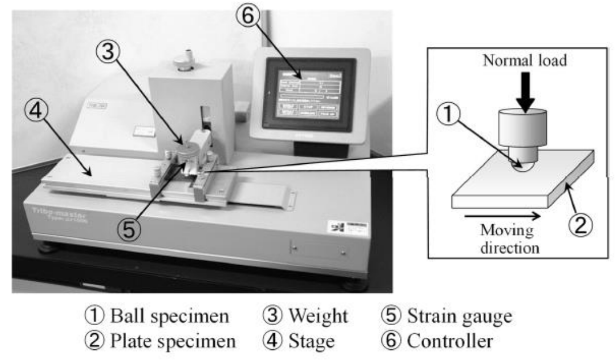
\includegraphics[width=100truemm,clip]{fig/fig_摩擦試験機.png}
    \caption{Schematic diagram of reciprocating sliding friction tester.}
    \label{fig:fig_摩擦試験機}
\end{figure}

\begin{table}[htbp]
    \centering
    \caption{Experimental conditions.}
    \label{tbl:実験条件}
    \scalebox{0.8}{
    \begin{tabular}{|l|ccc|}
    \hline
    ボール半径 R,mm                & \multicolumn{1}{c|}{1}    & \multicolumn{1}{c|}{4}    & 8     \\ \hline
    \multirow[c]{3}{*}{\centering 垂直荷重 W,N} & \multicolumn{1}{c|}{0.98} & \multicolumn{1}{c|}{0.98} & 0.098 \\ \cline{2-4} 
                              & \multicolumn{1}{c|}{4.9}  & \multicolumn{1}{c|}{4.9}  & 0.196 \\ \cline{2-4} 
                              & \multicolumn{1}{c|}{9.8}  & \multicolumn{1}{c|}{9.8}  & 0.49  \\ \hline
    すべり速度 v,mm/s              & \multicolumn{3}{c|}{1}                                        \\ \hline
    ストローク l,mm                & \multicolumn{3}{c|}{5}                                        \\ \hline
    同一条件の試行回数 N,cycles        & \multicolumn{3}{c|}{5}                                        \\ \hline
    潤滑状態                      & \multicolumn{3}{c|}{大気中無潤滑}                                   \\ \hline
    \end{tabular}
    }
\end{table}
    